% !TeX root = Bericht.tex
% !TeX spellcheck = de_DE
\section{Ergebnisse}
Es wurden Messungen bei 5 unterschiedlichen Beschleunigungsspannungen und konstantem Magnetfeld gemacht. Die statistischen Fehler der Strom- bzw. Spannungsmessung liegt in der letzten Nachkommastelle und spiegelt die Genauigkeit der Multimeter wieder. Für die Distanzmessungen wird ein Ablesefehler von \( 1 \unit{mm} \) angenommen. 

Aus den zwei Distanzmessungen \( d_1 \) und \( d_2 \) lässt sich der Radius \( r = \tfrac{d_2 - d_1}{2} \) der Kreisbahn bestimmen. Spannung und Strom wurden nach einstellen (also vor einem Dreierdurchgang an Messungen) notiert. Obwohl die Stromstärke manuell nicht verändert wurde, hat diese mit der Zeit abgenommen, da die Spulen sich aufheizen und den elektrischen Widerstand erhöhen (wodurch bei konstanter Spannung weniger Strom fließt). Aus dem Strom lässt sich gemäß \autoref{eqn:H} die Magnetfeldstärke \( B \) berechnen und man erhält Werte bei rund \( 800 \unit{\micro\tesla} \). 

Nach \autoref{eqn:e/m} hängt der quadratische Radius \( r^2 \) linear von der Beschleunigungsspannung \( U \) ab (multipliziert mit einer Konstanten \( k = 2/B^2 \)). Die Proportionalitätskonstante ist hierbei die spezifische Ladung vom Elektron \( e/m_{\text{e}} \). Deshalb wurde in \autoref{fig:fit} die gemessene Spannung mal der Konstanten \( k \) auf den quadratischen Radius aufgetragen. Da zu jeder Spannung 3 Messungen durchgeführt wurden (jeweils von anderen Personen), wird noch der Mittelwert gebildet (in rot zu sehen). Durch die gemittelten Daten wurde dann eine lineare Funktion der Form \( f(x) = ax \) angepasst. Ein Fit wurde mit allen gemittelten Daten durchgeführt (Fit 1), während für den zweiten Fit (Fit 2) der linkeste Datenpunkt nicht berücksichtigt wurde. 

\begin{figure}[H]	
	\centering
	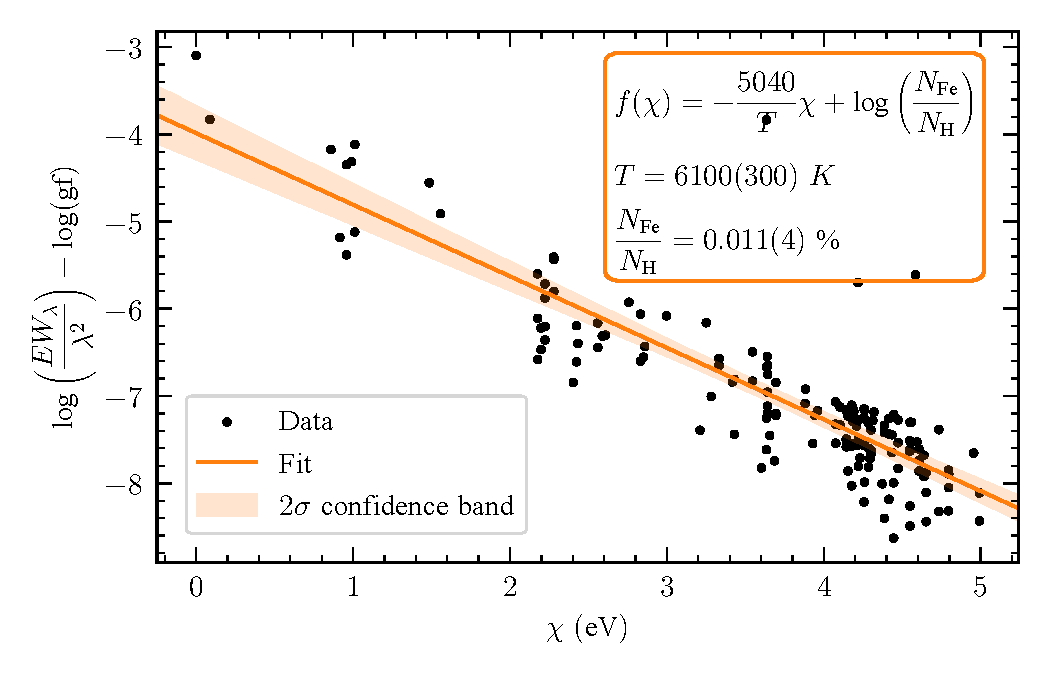
\includegraphics[width=\textwidth]{fit}
	\caption{In schwarz ist die eingestellte Spannung auf den gemessenen quadrierten Radius aufgetragen. In rot ist der Mittelwert der einzelnen Messreihen dargestellt. Dazu wurden zwei Geraden angepasst, für die grüne Linie wurden alle roten Datenpunkte berücksichtigt, während für die blaue der erste Datenpunkt nicht verwendet wurde. In hellblau ist das \( 95 \% \) Konfidenzband des blauen Fits zu sehen.}
	\label{fig:fit}
\end{figure}

Die Daten sind in beiden Richtungen fehlerbehaftet, der Spannungsfehler ist hierbei nur sehr gering und ist deshalb in der Abbildung nicht zu sehen. Für die Geradenanpassung wurde ODR (orthogonal distance regression \cite{odr}) verwendet, da die unabhängige Variable (auf der x-Achse) auch fehlerbehaftet ist und dies bei „gewöhnlichen” least-squares Fitroutinen nicht berücksichtigt wird. 
Für die Steigung der beiden Geraden ergibt sich einmal \( a_1 = 1.97(8) \cdot 10^{11} \unit{C/kg} \) für den Fit mit allen Datenpunkten und \( a_2 = 1.92(4) \cdot 10^{11} \unit{C/kg} \) für den zweiten Fit. Die Wahl, einen zweiten Fit ohne den inkonsistenten Datenpunkt durchzuführen kann man in dieser Darstellung der Daten noch nicht ganz motivieren, wird aber weiter unten diskutiert. Damit ergibt sich für die spezifische Ladung des Elektrons 

\begin{equation}
	\frac{e}{m_{\text{e}}} = a_2 = 1.92(4) \cdot 10^{11} \unit{C/kg}
\end{equation}


Im Vergleich zur spezifischen Ladung ist die wahrscheinlich interessantere Größe die Elementarladung \( e \). Dafür wurde die Elektronenmasse \( m_{\text{e}} \) dem CODATA 2018 Index entnommen \cite{codata} und mit allen anderen bekannten Größen in \autoref{eqn:e} eingesetzt; die einzige verbleibende Unbekannte ist die Elementarladung. In \autoref{fig:joyplot} wurde für alle Messungen die Elementarladung bestimmt und  als normalisierte Gaußkurve nach Namen des Durchführenden sortiert dargestellt. Das Analoge zum Fit ist hier die Überlagerung der 15 Normalverteilungen, um so einen besten Schätzwert zu erhalten. Hier wurden wieder einmal alle Gaußkurven kombiniert und einmal alle außer dem ganz rechten Messpunkt. 

\begin{figure}[H]	
	\centering
	\includegraphics[width=\textwidth]{joyplot}
	\caption{Die aus den Messungen berechnete Elementarladung ist als normalisierte Gaußkurve auf die 3 Versuchsteilnehmer getrennt aufgetragen. Auf der untersten Achse wurden die obigen Normalverteilungen kombiniert, wobei für die gelbe alle und für die pinke alle außer den roten Messpunkt miteinbezogen wurden.}
	\label{fig:joyplot}
\end{figure}

Man erkennt sehr gut, dass 4 der 5 Datenpunkte miteinander verträglich sind, während Messreihe 4 stark davon abweicht. Auch wenn Wahrscheinlichkeitsdichten nie 0 annehmen, ist es praktisch unmöglich, dass die 4 Messung per Zufall bei allen 3 Versuchsteilnehmern zu solchen Ergebnissen führt. Diese Darstellung motiviert die Wahl, in der Auswertung einen zweiten Fit ohne diesem Messpunkt durchzuführen.

Kombiniert man also die 4 konsistenten Messreihen (als gewichteten Mittelwert, bzw. als Überlagerung der Gaußkurven) erhält man für die Elementarladung einen Wert von \( e = 1.75(2) \cdot 10^{-19} \unit{C} \). Der statistische Fehler von \( e \) kommt zu über \( 90 \% \) aus den Distanzmessungen. Nimmt man an, dass die gemessenen Strom- bzw. Spannungswerte stimmen, kann man berechnen, was für ein Radius gemessen werden müsste, um auf den Literaturwert der Elementarladung zu kommen. Da stellt sich heraus, dass wir bei allen Messungen um \( 2 - 3 \unit{mm} \) (außer bei Messreihe 4 da sind es \( 9 \unit{mm} \)) systematisch darüber liegen. Die Systematik deutet eine leichte Abhängigkeit vom Radius an, kann aber nicht mit Sicherheit gesagt werden. Das motiviert die Suche nach möglichen systematischen Fehlern im Versuchsaufbau.


\subsection{Systematische Fehler}
In diesem Kapitel werden die identifizierten systematischen Messfehler abgeschätzt bzw. qualitativ diskutiert. Der erste diskutierte Fehler kommt durch das Magnetfeld zustande, das mit den zwei Spulen erzeugt wird. Für dieses nehmen wir im Zentrum homogene Eigenschaften an, jedoch sind diese nur in erster Näherung gegeben. Um eine bessere Abschätzung des Fehlers vorzunehmen wird das Magnetfeld simuliert und ist in \autoref{fig:helmholtz} dargestellt. Dabei stellen die Konturlinien die Magnetfeldlinien der Helmholtzspule dar. In einem homogenen Magnetfeld würden diese in der Mitte parallel mit möglichst großen Abstand sein. Durch eine qualitative Betrachtung der Abbildung wird von einer guten Näherung ausgegangen. 

\begin{figure}[H]
	\includegraphics[width=\textwidth]{helmholtz}
	\caption{Zeigt das Magnetfeld, welches von der Helmholtzspule erzeugt wird. Dabei sind die Konturlinien die Magnetfeldlinien. In schwarz sind die zwei Spulen und der Tisch angedeutet.}
	\label{fig:helmholtz}
\end{figure}

\noindent Ein weiterer geometrischer Fehler vom Aufbau liegt in der Lichtbrechung. Wenn Licht von einen Medium in ein Zweites übergeht wird dieses am Übergang gebrochen. Dieser Effekt spielt in unserem Experiment beim Übergang von Luft auf Glas und im gleichen Maße wieder beim Übergang Glas zu nahezu Vakuum eine Rolle. 

Da Luft und dünnes Wasserstoffgas einen nahezu identen Brechungsindex haben, kann der Lichtstrahl in Luft und im Kolben als parallel angesehen werden. Im Glas kommt es also zu einer Verschiebung normal zur Ausbreitungsrichtung. Die Verschiebung wird in Abhängigkeit vom Kolbenmittelpunkt für eine Glasstärke von \( 2 \unit{mm} \) in \autoref{fig:systematischeFehler} auf der linken Seite gezeigt.

Zusätzlich wurde auch der Winkel des Spiegels als potentielle systematische Fehlerquelle identifiziert. Wenn dieser nicht normal zum Magnetfeld steht, kann es zu Projektionsfehlern kommen, welche die Messung des Radius verzerren. Eine Abschätzung der Größe ist in Abbildung \ref{fig:systematischeFehler} auf der linken Seite gegeben. 

\begin{figure}[H]
	\includegraphics[width=\textwidth]{systematischeFehler}
	\caption{Abschätzung von Möglichen systematischen Fehlern. Durch die Brechung von Licht am Glas entsteht eine Verschiebung des Lichtstrahles, wie in der linken Graphik zu erkennen ist. Auf der rechten Seite ist der Projektionsfehler über den Winkel des Spiegels abgeschätzt.}
	\label{fig:systematischeFehler}
\end{figure}

Während die Lichtbrechung den systematischen Fehler vergrößert (also zu einer noch größere Abweichung vom Literaturwert führt), kann durch die nichtparallelität je nach Richtung den Fehler vergrößern und verkleinern. Dabei können schon kleine Winkel zu signifikanten Verschiebungen der Position kommen. Nimmt man für die Lichtbrechung einen maximalen Fehler von \( 2 \unit{mm} \) an (wir liegen dann \( 4 - 5 \unit{mm} \) vom erwarteten Radius entfernt) kann das mit nur \( 2 - 3 \unit{°} \) wieder wettgemacht werden. 






















